\section{Wojciech Dudek}
\label{sec:wojdud}

To je zaawansowanna matematyka prosze państwa
\begin{math}
\\a = F*m
\\(a+b)^2 = a^2 + 2ab + b^2
\end{math}

\begin{figure}[htbp]
    \centering   
    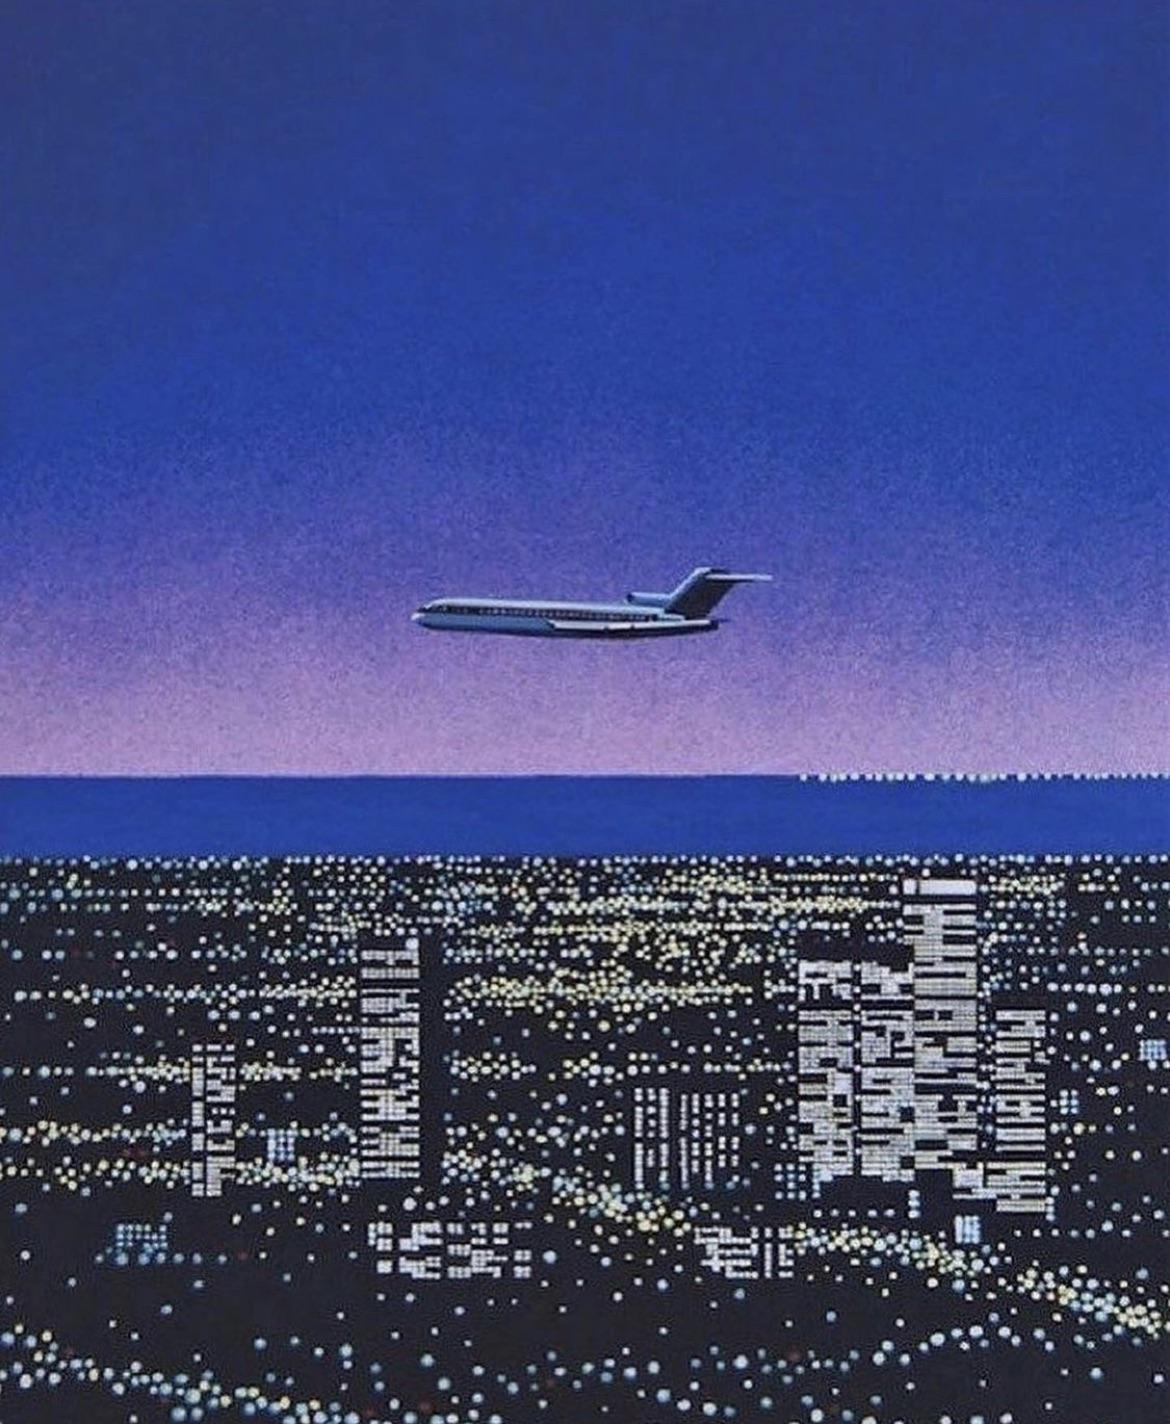
\includegraphics[width=0.4\textwidth]{pictures/fotalatex.jpg}
    \caption{Obraz Hiroshi Nagai'ego}
    \label{fig:animuobrazek}
\end{figure}

Tabela ~\ref{tab:tabwojdud} ukazuje jakieś elementy które tam wpisałem.

\begin{table}[htbp]
\centering
\begin{tabular}{| c | c | c | c | c |}
    \hline
     & col1 & col2 & col3 & col4 \\
    \hline
    w1 & b    & c    & d    & e    \\
    w2 & g    & h    & i    & j    \\
    w3 & k    & l    & m    & n    \\
    \hline
\end{tabular}
\caption{Tabela mocy}
\label{tab:tabwojdud}
\end{table}



To jest lista nienumerowana
\begin{itemize}
    \item rower
    \item samochód
    \item hulajduszanogapiekłaniema
    \item nudzimiesie
    \item next
\end{itemize}

To jest lista numerowana
\begin{enumerate}
    \item pierwszy element
    \item drugi element
    \item trzeci element
\end{enumerate}

To jest krótki tekst z odniesieniami:

Przyjechali kowboje każdy pali swoje!
Przyjechali \textbf{bandyci} każdy \textit{pali} co chyci!
\textbf{Uga buga \emph{kto da} szluga?}\\ 
Patrząc na obraz \ref{fig:animuobrazek} można zauważyć samolot\\
Jak pokazują dane w tabeli \ref{tab:tabwojdud} nie wiadomo o co chodzi.
